\documentclass[hyperref={},
xcolor={dvipsnames,svgnames,table},10pt]{beamer}
\usepackage{concrete} 
\usepackage{amsmath}
\usepackage{tikz}
\usepackage{algorithm}
\usepackage{algorithmic}
\usepackage[utf8]{inputenc}
\usepackage[T1]{fontenc}
\usepackage{pdfpages} 
\usepackage{multirow}
\usetheme{Warsaw}
\usepackage[frenchb]{babel}
\setlength\parindent{0pt}
%\setbeamertemplate{navigation symbols}{}



\title{TER Sur Le Problème Des Préflots}
\author{DUVILLIE Guillerme \\ Ould Mohamed Abdellahi Cheikh Mehdi}
\institute{Université Montpellier2\\ Master1-Informatique\\ Spécialité-MOCA}
\logo{
\includegraphics[scale=0.2]{Logo_UM2.png}}


\begin{document}

\begin{frame}
	\titlepage 
\end{frame}

\AtBeginSection[]
{
	\begin{frame}<beamer>
		\frametitle{Plan}
		\tableofcontents[currentsection]
	\end{frame}
}

\begin{frame}{Sommaire}
  \tableofcontents
\end{frame} 

\section{Introduction : le flot et ses algorithmes}

\subsection{Cadre du TER}
\begin{frame}{Cadre et objectifs}
	\begin{itemize}
		\item Ce TER se situe dans le cadre de Problème de flot maximum

		\item Il existe différents types d'algorithmes répondant à ce problème, certains basés sur la recherche
			de chaînes améliorantes (Edmonds-Karp, Ford Fulkerson, ...), d'autres sur les fonctions de préflots. 
			Nous nous intéresserons à la seconde catégorie.
	\end{itemize}
\end{frame}

\subsection{Motivation}
\begin{frame}{Utilité}
	
	Considérons une entreprise, devant acheminer sa production depuis
	l'usine de création au lieu de stockage. \vfill

	\begin{center}
		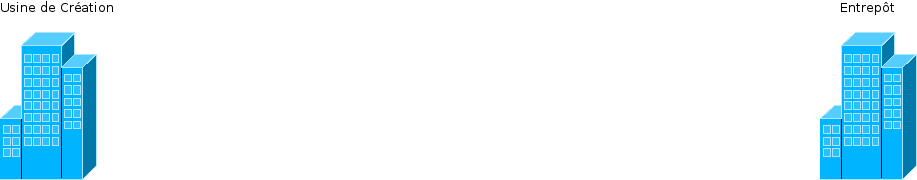
\includegraphics[scale=0.32]{img/etape1.png}
	\end{center}
\end{frame}

\begin{frame}{Utilité}
	Il existe différents points, par lesquels peut transiter la production.

	\begin{center}
		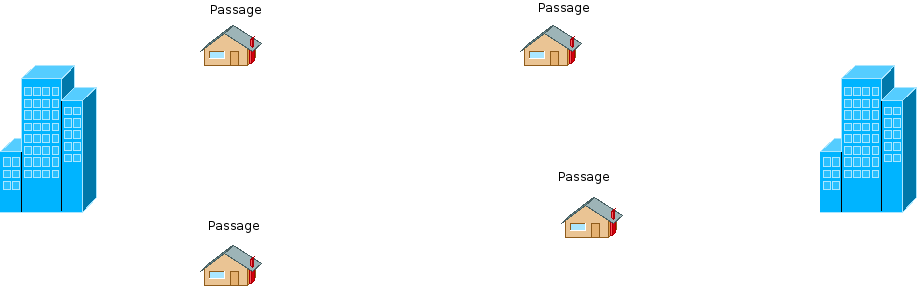
\includegraphics[scale=0.32]{img/etape2.png}
	\end{center}
\end{frame}

\begin{frame}{Utilité}
	Chaque passage est reliés aux autres à l'aide de routes permettant un transit plus ou moins facile
	jusqu'à destination.

	\begin{center}
		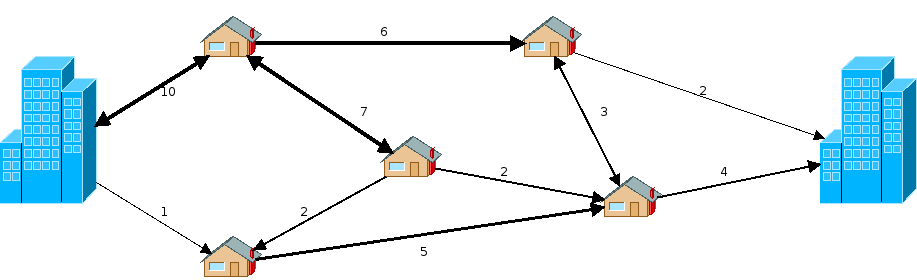
\includegraphics[scale=0.32]{img/exemple.png}
	\end{center}
\end{frame}

\begin{frame}{Utilité}
	Chaque passage est reliés aux autres à l'aide de routes permettant un transit plus ou moins facile
	jusqu'à destination.

	\begin{center}
		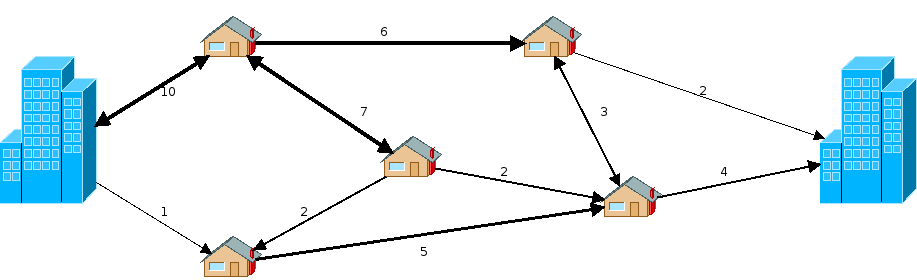
\includegraphics[scale=0.32]{img/exemple.png}
	\end{center}

	\begin{alertblock}{Bingo!}
		Il s'agit là d'un problème de flot maximum.
	\end{alertblock}
\end{frame}

\subsection{Les algorithmes de chaînes améliorantes}
\begin{frame}{Définitions}
		Nous allons définir quelques notions qui seront utlisées par la suite
		pour le déroulement de l'algorithme de préflot et ses dérivés.
\end{frame}

\begin{frame}{La notion de flot}
	Un flot est une fonction de graphes vérifiant certaines propriétés, qui sont : \vfill \vfill
\end{frame} 

\begin{frame}{La notion de flot}
	Un flot est une fonction de graphes vérifiant certaines propriétés, qui sont : ~\\~\\
	\begin{exampleblock}{le respect de la capacité de l'arc}
		La valeur du flot sur un arc ne peut être supérieure à la capacité de l'arc et ne peut être négative
	\end{exampleblock}\vfill
\end{frame} 

\begin{frame}{La notion de flot}
	Un flot est une fonction de graphes vérifiant certaines propriétés, qui sont :~\\~\\
	\begin{block}{le respect de la capacité de l'arc}
		$$\forall (i,j) \in A, \quad 0 \leq x(i,j) \leq c(i,j)$$
	\end{block}\vfill
	\begin{exampleblock}{le respect de la loi de Kirchoff}
		Pour chaque noeud différent de la source et du puits, la quantité de flot entrant dans le noeud
		est égale à la quantité de flot sortant de ce dernier.
	\end{exampleblock}\vfill
\end{frame} 

\begin{frame}{La notion de flot}
	Un flot est une fonction de graphes vérifiant certaines propriétés, qui sont : 
	\begin{block}{le respect de la capacité de l'arc}
		$$\forall (i,j) \in A, \quad 0 \leq x(i,j) \leq c(i,j)$$
	\end{block}\vfill
	\begin{block}{le respect de la loi de Kirchoff}
		$$\forall i \in S - \{s,t\}, \quad \sum_{j \in A^+(i)} x(i,j) = \sum_{k\in A^-(i)} x(k,i)$$
	\end{block}\vfill
	\begin{exampleblock}{Le respect de la contrainte de symétrie}
		Pour chaque arc du graphe, il n'y a aucun phénomène de perte entre le sommet de départ et le
		sommet d'arrivée.
	\end{exampleblock}\vfill
\end{frame} 

\begin{frame}{La notion de flot}
	Un flot est une fonction de graphes vérifiant certaines propriétés, qui sont : 
	\begin{block}{le respect de la capacité de l'arc}
		$$\forall (i,j) \in A, \quad 0 \leq x(i,j) \leq c(i,j)$$
	\end{block}\vfill
	\begin{block}{le respect de la loi de Kirchoff}
		$$\forall i \in S - \{s,t\}, \quad \sum_{j \in A^+(i)} x(i,j) = \sum_{k\in A^-(i)} x(k,i)$$
	\end{block}\vfill
	\begin{block}{Le respect de la contrainte de symétrie}
		$$ f = \sum_{j \in A^+(s)} x(s,j) = \sum_{k\in A^- (t)} x(k,t) $$ 
	\end{block}\vfill
\end{frame} 

\begin{frame}{Le réseau résiduel}
 	Soit un graphe $G(S, A)$, un flot $f$ et $i,j$ deux sommets de $G$. On dira que
	l'arête $(i,j)$ appartiendra au réseau résiduel $A_f$ si et seulement si la capacité résiduelle
	est non nulle.

	\begin{alertblock}{Autrement dit}
	 	$$ r(i,j) = c(i,j) - x(i,j) > 0 $$ 
	\end{alertblock}

	On appelle alors $r(i,j)$ la capacité résiduelle de l'arête $(i,j)$. 
	\vfill
\end{frame}

\begin{frame}{Le réseau résiduel}
 	Soit un graphe $G(S, A)$, un flot $f$ et $i,j$ deux sommets de $G$. On dira que
	l'arête $(i,j)$ appartiendra au réseau résiduel $A_f$ si et seulement si la capacité résiduelle
	est non nulle.

	\begin{alertblock}{Autrement dit}
	 	$$ r(i,j) = c(i,j) - x(i,j) > 0 $$ 
	\end{alertblock}


	On appelle alors $r(i,j)$ la capacité résiduelle de l'arête $(i,j)$. 

	\begin{block}{Note}
		Si $x(i,j) > 0$ alors $(j,i)$ appartient au réseau résiduel avec une capacité résiduelle $r(j,i) = x(i,j)$.
	\end{block}
\end{frame}

\begin{frame}{Le réseau résiduel}
 	Soit un graphe $G(S, A)$, un flot $f$ et $i,j$ deux sommets de $G$. On dira que
	l'arête $(i,j)$ appartiendra au réseau résiduel $A_f$ si et seulement si la capacité résiduelle
	est non nulle.

	\begin{alertblock}{Autrement dit}
	 	$$ r(i,j) = c(i,j) - x(i,j) > 0 $$ 
	\end{alertblock}


	On appelle alors $r(i,j)$ la capacité résiduelle de l'arête $(i,j)$. 

	\begin{alertblock}{Théorème}
	S'il existe un chemin de la source au puits dans le réseau résiduel, alors on peut augmenter la
	valeur du flot dans le graphe. Ce chemin est appelé chaîne améliorante.
	\end{alertblock}
\end{frame}

\begin{frame}{Le réseau résiduel}
	Pour le flot suivant, ... \vfill
	\begin{minipage}[c]{0.45\linewidth}
		\begin{figure}
			\begin{tikzpicture}[scale=0.7]
				\tikzset{noeud/.style={circle, draw=black, inner sep=0.1cm, minimum width=0.6cm}, fleche/.style={>=latex, ->}};
				\node[noeud] (s) at (0,0) {s};
				\node[noeud] (a) at (2, 2) {a};
				\node[noeud] (b) at (2, -2) {b};
				\node[noeud] (c) at (4.5, -2) {c};
				\node[noeud] (d) at (4.5, 2) {d};
				\node[noeud] (t) at (6.5,0) {t};

				\draw[fleche, red] (s) -- node[above left, red] {$2/2$}(a);
				\draw[fleche] (s) -- node[below left] {$0/1$}(b);
				\draw[fleche, red] (a) -- node[left,red] {$1/1$}(b);
				\draw[fleche, red] (a) -- node[above, red] {$1/3$}(d);
				\draw[fleche] (d) -- node[above left] {$0/1$}(b);
				\draw[fleche, red] (b) -- node[below, red] {$1/1$}(c);
				\draw[fleche, red] (d) -- node[above right, red] {$1/4$}(t);
				\draw[fleche, red] (c) -- node[below right, red] {$1/1$}(t);
				\draw[fleche] (c) -- node[right] {$0/2$}(d);
			\end{tikzpicture}
			\caption{Un exemple de flot}
		\end{figure}
	\end{minipage} \hfill
	\begin{minipage}[c]{0.45\linewidth}
	\end{minipage}
\end{frame}

\begin{frame}{Le réseau résiduel}
	$\dots$ on a le réseau résiduel suivant : \vfill
	\begin{minipage}[c]{0.45\linewidth}
		\begin{figure}
			\begin{tikzpicture}[scale=0.7]
				\tikzset{noeud/.style={circle, draw=black, inner sep=0.1cm, minimum width=0.6cm}, fleche/.style={>=latex, ->}};
				\node[noeud] (s) at (0,0) {s};
				\node[noeud] (a) at (2, 2) {a};
				\node[noeud] (b) at (2, -2) {b};
				\node[noeud] (c) at (4.5, -2) {c};
				\node[noeud] (d) at (4.5, 2) {d};
				\node[noeud] (t) at (6.5,0) {t};

				\draw[fleche, red] (s) -- node[above left, red] {$2/2$}(a);
				\draw[fleche] (s) -- node[below left] {$0/1$}(b);
				\draw[fleche, red] (a) -- node[left,red] {$1/1$}(b);
				\draw[fleche, red] (a) -- node[above, red] {$1/3$}(d);
				\draw[fleche] (d) -- node[above left] {$0/1$}(b);
				\draw[fleche, red] (b) -- node[below, red] {$1/1$}(c);
				\draw[fleche, red] (d) -- node[above right, red] {$1/4$}(t);
				\draw[fleche, red] (c) -- node[below right, red] {$1/1$}(t);
				\draw[fleche] (c) -- node[right] {$0/2$}(d);
			\end{tikzpicture}
			\caption{Un exemple de flot}
		\end{figure}
	\end{minipage} \hfill
	\begin{minipage}[c]{0.45\linewidth}
		\begin{figure}
			\begin{tikzpicture}[scale=0.7]
				\tikzset{noeud/.style={circle, draw=black, inner sep=0.1cm, minimum width=0.6cm}, fleche/.style={>=latex, ->}};
				\node[noeud] (s) at (0,0) {s};
				\node[noeud] (a) at (2, 2) {a};
				\node[noeud] (b) at (2, -2) {b};
				\node[noeud] (c) at (4.5, -2) {c};
				\node[noeud] (d) at (4.5, 2) {d};
				\node[noeud] (t) at (6.5,0) {t};

				\draw[fleche, purple] (a) -- node[above left, purple] {$2$}(s);
				\draw[fleche] (s) -- node[below left] {$1$}(b);
				\draw[fleche, purple] (b) -- node[left, purple] {$1$}(a);
				\draw[fleche] (a) to[out=15, in=165]  node[above] {$2$}(d);
				\draw[fleche, purple] (d) to[out=195, in=345]  node[below, purple] {$1$}(a);
				\draw[fleche] (d) -- node[below right] {$1$}(b);
				\draw[fleche, purple] (c) -- node[below, purple] {$1$}(b);
				\draw[fleche] (d) to[out=295, in=145] node[below left] {$3$}(t);
				\draw[fleche, purple] (t) to[out=115, in=335] node[above right, purple] {$1$}(d);
				\draw[fleche, purple] (t) -- node[below right, purple] {$1$}(c);
				\draw[fleche] (c) -- node[right] {$2$}(d);
			\end{tikzpicture}
			\caption{Le réseau résiduel associé}
		\end{figure}
	\end{minipage}
\end{frame}

\begin{frame}{Le réseau résiduel}
Il existe une chaîne améliorante dans le graphe d'écart : \vfill
	\begin{minipage}[c]{0.45\linewidth}
		\begin{figure}
			\begin{tikzpicture}[scale=0.7]
				\tikzset{noeud/.style={circle, draw=black, inner sep=0.1cm, minimum width=0.6cm}, fleche/.style={>=latex, ->}};
				\node[noeud] (s) at (0,0) {s};
				\node[noeud] (a) at (2, 2) {a};
				\node[noeud] (b) at (2, -2) {b};
				\node[noeud] (c) at (4.5, -2) {c};
				\node[noeud] (d) at (4.5, 2) {d};
				\node[noeud] (t) at (6.5,0) {t};

				\draw[fleche, red] (s) -- node[above left, red] {$2/2$}(a);
				\draw[fleche] (s) -- node[below left] {$0/1$}(b);
				\draw[fleche, red] (a) -- node[left,red] {$1/1$}(b);
				\draw[fleche, red] (a) -- node[above, red] {$1/3$}(d);
				\draw[fleche] (d) -- node[above left] {$0/1$}(b);
				\draw[fleche, red] (b) -- node[below, red] {$1/1$}(c);
				\draw[fleche, red] (d) -- node[above right, red] {$1/4$}(t);
				\draw[fleche, red] (c) -- node[below right, red] {$1/1$}(t);
				\draw[fleche] (c) -- node[right] {$0/2$}(d);
			\end{tikzpicture}
			\caption{Un exemple de flot}
		\end{figure}
	\end{minipage} \hfill
	\begin{minipage}[c]{0.45\linewidth}
		\begin{figure}
			\begin{tikzpicture}[scale=0.7]
				\tikzset{noeud/.style={circle, draw=black, inner sep=0.1cm, minimum width=0.6cm}, fleche/.style={>=latex, ->}};
				\node[noeud] (s) at (0,0) {s};
				\node[noeud] (a) at (2, 2) {a};
				\node[noeud] (b) at (2, -2) {b};
				\node[noeud] (c) at (4.5, -2) {c};
				\node[noeud] (d) at (4.5, 2) {d};
				\node[noeud] (t) at (6.5,0) {t};

				\draw[fleche] (a) -- node[above left] {$2$}(s);
				\draw[fleche, orange] (s) -- node[below left, orange] {$1$}(b);
				\draw[fleche, orange] (b) -- node[left, orange] {$1$}(a);
				\draw[fleche, orange] (a) to[out=15, in=165]  node[above, orange] {$2$}(d);
				\draw[fleche] (d) to[out=195, in=345]  node[below] {$1$}(a);
				\draw[fleche] (d) -- node[below right] {$1$}(b);
				\draw[fleche] (c) -- node[below] {$1$}(b);
				\draw[fleche, orange] (d) to[out=295, in=145] node[below left, orange] {$3$}(t);
				\draw[fleche] (t) to[out=115, in=335] node[above right] {$1$}(d);
				\draw[fleche] (t) -- node[below right] {$1$}(c);
				\draw[fleche] (c) -- node[right] {$2$}(d);
			\end{tikzpicture}
			\caption{Le réseau résiduel associé}
		\end{figure}
	\end{minipage}
\end{frame}

\begin{frame}{Le réseau résiduel}
	Donc une augmentation possible du flot : \vfill
	\begin{minipage}[c]{0.45\linewidth}
		\begin{figure}
			\begin{tikzpicture}[scale=0.7]
				\tikzset{noeud/.style={circle, draw=black, inner sep=0.1cm, minimum width=0.6cm}, fleche/.style={>=latex, ->}};
				\node[noeud] (s) at (0,0) {s};
				\node[noeud] (a) at (2, 2) {a};
				\node[noeud] (b) at (2, -2) {b};
				\node[noeud] (c) at (4.5, -2) {c};
				\node[noeud] (d) at (4.5, 2) {d};
				\node[noeud] (t) at (6.5,0) {t};

				\draw[fleche, red] (s) -- node[above left, red] {$2/2$}(a);
				\draw[fleche, red] (s) -- node[below left, red] {$1/1$}(b);
				\draw[fleche] (a) -- node[left] {$0/1$}(b);
				\draw[fleche, red] (a) -- node[above, red] {$2/3$}(d);
				\draw[fleche] (d) -- node[above left] {$0/1$}(b);
				\draw[fleche, red] (b) -- node[below, red] {$1/1$}(c);
				\draw[fleche, red] (d) -- node[above right, red] {$2/4$}(t);
				\draw[fleche, red] (c) -- node[below right, red] {$1/1$}(t);
				\draw[fleche] (c) -- node[right] {$0/2$}(d);
			\end{tikzpicture}
			\caption{Un exemple de flot}
		\end{figure}
	\end{minipage} \hfill
	\begin{minipage}[c]{0.45\linewidth}
		\begin{figure}
			\begin{tikzpicture}[scale=0.7]
				\tikzset{noeud/.style={circle, draw=black, inner sep=0.1cm, minimum width=0.6cm}, fleche/.style={>=latex, ->}};
				\node[noeud] (s) at (0,0) {s};
				\node[noeud] (a) at (2, 2) {a};
				\node[noeud] (b) at (2, -2) {b};
				\node[noeud] (c) at (4.5, -2) {c};
				\node[noeud] (d) at (4.5, 2) {d};
				\node[noeud] (t) at (6.5,0) {t};

				\draw[fleche] (a) -- node[above left] {$2$}(s);
				\draw[fleche, orange] (s) -- node[below left, orange] {$1$}(b);
				\draw[fleche, orange] (b) -- node[left, orange] {$1$}(a);
				\draw[fleche, orange] (a) to[out=15, in=165]  node[above, orange] {$2$}(d);
				\draw[fleche] (d) to[out=195, in=345]  node[below] {$1$}(a);
				\draw[fleche] (d) -- node[below right] {$1$}(b);
				\draw[fleche] (c) -- node[below] {$1$}(b);
				\draw[fleche, orange] (d) to[out=295, in=145] node[below left, orange] {$3$}(t);
				\draw[fleche] (t) to[out=115, in=335] node[above right] {$1$}(d);
				\draw[fleche] (t) -- node[below right] {$1$}(c);
				\draw[fleche] (c) -- node[right] {$2$}(d);
			\end{tikzpicture}
			\caption{Le réseau résiduel associé}
		\end{figure}
	\end{minipage}
\end{frame}

\begin{frame}{Les algorithmes}
	Varient sur le choix des chaînes améliorantes : \vfill
\end{frame}

\begin{frame}{Les algorithmes}
	Varient sur le choix des chaînes améliorantes : \vfill
	\begin{itemize}
		\item \underline{Ford-Fulkerson} : choix aléatoire \vfill
	\end{itemize}
\end{frame}

\begin{frame}{Les algorithmes}
	Varient sur le choix des chaînes améliorantes : \vfill
	\begin{itemize}
		\item \underline{Ford-Fulkerson} : choix aléatoire \vfill
		\item \underline{Edmonds-Karp} : la plus petite chaîne en nombre d'arcs\vfill
	\end{itemize}
\end{frame}

\begin{frame}{Les algorithmes}
	Varient sur le choix des chaînes améliorantes : \vfill
	\begin{itemize}
		\item \underline{Ford-Fulkerson} : choix aléatoire \vfill
		\item \underline{Edmonds-Karp} : la plus petite chaîne en nombre d'arcs\vfill
		\item \underline{Dinic} : l'ensemble des plus petites chaînes en nombre d'arcs \vfill
	\end{itemize}
\end{frame}

\begin{frame}{Les limites de ces algorithmes}
	Considérons le graphe suivant :\vfill

	\begin{figure}
	\begin{center}
	\scalebox{0.6}{
		\begin{tikzpicture}
			\tikzset{noeud/.style={circle, draw=black, text centered,minimum size=26pt, inner sep=0pt},
			fleche/.style={thick}};

			\node[noeud] (t) at (12, 0) {$t$};
			\node[noeud] (s) at (0, 0) {$s$};
			\node[noeud] (1) at (2, 0) {$1$};

			\foreach \x in {2, 3, 4, 5}{
				\node[noeud] (\x) at (2*\x, 0) {$\x$}; 
			}

			\node[noeud] (6) at ( 9, 1) {$7$};
			\node[noeud] (7) at (11, 1) {$8$};
			\node[noeud] (8) at (8.5, 2) {$9$};
			\node[noeud] (9) at (10, 2.5) {$10$};
			\node[noeud] (10) at (11.5, 2) {$11$};
			\node (p1) at (8.5, 3) {$\vdots$};
			\node (p2) at (11.5, 3) {$\vdots$};
			\node[noeud] (k) at (7, 4) {$k$};
			\node (p3) at (10, 4.5) {$\dots$};
			\node[noeud] (n) at (13, 4) {$n-2$};

			\draw[fleche] (s) to node[below] {$\infty$} (1);
			\draw[fleche] (1) to node[below] {$\infty$} (2);
			\draw[fleche] (2) to node[below] {$\infty$} (3);
			\draw[fleche] (3) to node[below] {$\infty$} (4);
			\draw[fleche] (4) to node[below] {$\infty$} (5);
			\draw[fleche] (5) to node[below] {$\infty$} (t);

			\draw[fleche] (4) to node[above] {$1$} (6);
			\draw[fleche] (4) to node[above left] {$1$} (8);
			\draw[fleche] (4) to node[left] {$1$} (k);

			\draw[fleche] (n) to node[right] {$1$} (t);
			\draw[fleche] (7) to node[above right] {$1$} (t);
			\draw[fleche] (10) to node[right] {$1$} (t);

			\draw[fleche] (6) to node[above] {$1$} (7);
			\draw[fleche] (8) to node[above] {$1$} (9);
			\draw[fleche] (9) to node[above] {$1$} (10);

			\draw[fleche] (k) to node[above left] {$1$} (p3);
			\draw[fleche] (p3) to node[above right] {$1$} (n);
		\end{tikzpicture}}
	\end{center}
\end{figure} \vfill
\end{frame}

\begin{frame}{Introduction aux opérations}
	Considérons le graphe suivant :\vfill

	\begin{figure}
	\begin{center}
	\scalebox{0.6}{
		\begin{tikzpicture}
			\tikzset{noeud/.style={circle, draw=black, text centered,minimum size=26pt, inner sep=0pt},
			fleche/.style={thick}};

			\node[noeud] (t) at (12, 0) {$t$};
			\node[noeud] (s) at (0, 0) {$s$};
			\node[noeud] (1) at (2, 0) {$1$};

			\foreach \x in {2, 3, 4, 5}{
				\node[noeud] (\x) at (2*\x, 0) {$\x$}; 
			}

			\node[noeud] (6) at ( 9, 1) {$7$};
			\node[noeud] (7) at (11, 1) {$8$};
			\node[noeud] (8) at (8.5, 2) {$9$};
			\node[noeud] (9) at (10, 2.5) {$10$};
			\node[noeud] (10) at (11.5, 2) {$11$};
			\node (p1) at (8.5, 3) {$\vdots$};
			\node (p2) at (11.5, 3) {$\vdots$};
			\node[noeud] (k) at (7, 4) {$k$};
			\node (p3) at (10, 4.5) {$\dots$};
			\node[noeud] (n) at (13, 4) {$n-2$};

			\draw[fleche] (s) to node[below] {$\infty$} (1);
			\draw[fleche] (1) to node[below] {$\infty$} (2);
			\draw[fleche] (2) to node[below] {$\infty$} (3);
			\draw[fleche] (3) to node[below] {$\infty$} (4);
			\draw[fleche] (4) to node[below] {$\infty$} (5);
			\draw[fleche] (5) to node[below] {$\infty$} (t);

			\draw[fleche] (4) to node[above] {$1$} (6);
			\draw[fleche] (4) to node[above left] {$1$} (8);
			\draw[fleche] (4) to node[left] {$1$} (k);

			\draw[fleche] (n) to node[right] {$1$} (t);
			\draw[fleche] (7) to node[above right] {$1$} (t);
			\draw[fleche] (10) to node[right] {$1$} (t);

			\draw[fleche] (6) to node[above] {$1$} (7);
			\draw[fleche] (8) to node[above] {$1$} (9);
			\draw[fleche] (9) to node[above] {$1$} (10);

			\draw[fleche] (k) to node[above left] {$1$} (p3);
			\draw[fleche] (p3) to node[above right] {$1$} (n);
		\end{tikzpicture}}
	\end{center}
\end{figure} \vfill
\begin{alertblock}{Constat}
Il met en défaut les algorithmes de recherche de chaînes améliorantes.
\end{alertblock}
\end{frame}

\begin{frame}{Introduction aux opérations}
	Considérons le graphe suivant :\vfill

	\begin{figure}
	\begin{center}
	\scalebox{0.6}{
		\begin{tikzpicture}
			\tikzset{noeud/.style={circle, draw=black, text centered,minimum size=26pt, inner sep=0pt},
			fleche/.style={thick}};

			\node[noeud] (t) at (14, 0) {$t$};
			\node[noeud] (s) at (2, 0) {$s$};

			\foreach \x in {2, 3, 4, 5}{
				\node[noeud] (\x) at (2*\x, 0) {$\x$}; 
			}

			\foreach \y/\ytext in {3.5/6, 1.7/7, -1.7/n-1, -3.5/n}{
				\node[noeud] (\ytext) at (12, \y) {$\ytext$};
				\draw[fleche] (5) --node[right] {$1$} (\ytext) --node[left] {$1$} (t);
			}

			\node (point) at (12, 0) {$\vdots$};

			\draw[fleche] (s) --node[above] {$\infty$} (2) --node[above] {$\infty$} (3) --node[above] {$\infty$}
			(4) --node[above] {$\infty$} (5) ;

		\end{tikzpicture}}
	\end{center}
\end{figure} \vfill
\begin{exampleblock}{Intuition}
Agir de façon locale au noeud $5$, afin d'envoyer du flot à tous ses voisins en une seule opération.
\end{exampleblock}
\end{frame}





\section{Le préflot et ses algorithmes}


\begin{frame}{Intuitivement...}
	Le graphe est assimilé à un réseau de tuyaux de capacité donnée.\vfill
\end{frame}

\begin{frame}{Intuitivement...}
	Le graphe est assimilé à un réseau de tuyaux de capacité donnée.\vfill
	Chaque noeud possède un réservoir de capacité infinie.\vfill
\end{frame}

\begin{frame}{Intuitivement...}
	Le graphe est assimilé à un réseau de tuyaux de capacité donnée.\vfill
	Chaque noeud possède un réservoir de capacité infinie.\vfill
	Seule la source possède un réservoir plein. \vfill
\end{frame}

\begin{frame}{Intuitivement...}
	Le graphe est assimilé à un réseau de tuyaux de capacité donnée.\vfill
	Chaque noeud possède un réservoir de capacité infinie.\vfill
	Seule la source possède un réservoir plein. \vfill
	À chaque noeud est associée une hauteur.\vfill
\end{frame}

\begin{frame}{Intuitivement...}
	Le graphe est assimilé à un réseau de tuyaux de capacité donnée.\vfill
	Chaque noeud possède un réservoir de capacité infinie.\vfill
	Seule la source possède un réservoir plein. \vfill
	À chaque noeud est associée une hauteur.\vfill
	Deux actions possibles : \begin{enumerate}
		\item vidange du réservoir
	\end{enumerate} \vfill
\end{frame}

\begin{frame}{Intuitivement...}
	Le graphe est assimilé à un réseau de tuyaux de capacité donnée.\vfill
	Chaque noeud possède un réservoir de capacité infinie.\vfill
	Seule la source possède un réservoir plein. \vfill
	À chaque noeud est associée une hauteur.\vfill
	Deux actions possibles : \begin{enumerate}
		\item vidange du réservoir
		\item augmentation de la hauteur du réservoir
	\end{enumerate} \vfill
\end{frame}

\begin{frame}{Intuitivement...}
	Le graphe est assimilé à un réseau de tuyaux de capacité donnée.\vfill
	Chaque noeud possède un réservoir de capacité infinie.\vfill
	Seule la source possède un réservoir plein. \vfill
	À chaque noeud est associée une hauteur.\vfill
	Deux actions possibles : \begin{enumerate}
		\item vidange du réservoir
		\item augmentation de la hauteur du réservoir
	\end{enumerate} \vfill
	On commence par vidanger la source, puis on cherche à vidanger les noeuds dont le réservoir n'est
	pas vide. \vfill
\end{frame}

\begin{frame}{Intuitivement...}
	Le graphe est assimilé à un réseau de tuyaux de capacité donnée.\vfill
	Chaque noeud possède un réservoir de capacité infinie.\vfill
	Seule la source possède un réservoir plein. \vfill
	À chaque noeud est associée une hauteur.\vfill
	Deux actions possibles : \begin{enumerate}
		\item vidange du réservoir
		\item augmentation de la hauteur du réservoir
	\end{enumerate} \vfill
	On commence par vidanger la source, puis on cherche à vidanger les noeuds dont le réservoir n'est
	pas vide. \vfill
	Si on ne peut vidanger aucun réservoir et qu'il reste des réservoirs non vides, on augmente la
	hauteur de ces derniers. \vfill
\end{frame}


\subsection{Définitions}
\begin{frame}{La notion de préflot}
	Un préflot est une fonction obtenue à partir d'un flot par relaxation de la loi de Kirchoff : la
	quantité de préflot sortant d'un noeud doit être inférieure ou égale à la quantité de préflot
	entrant dans celui-ci.\vfill
\end{frame}

\begin{frame}{La notion de préflot}
	Un préflot est une fonction obtenue à partir d'un flot par relaxation de la loi de Kirchoff : la
	quantité de préflot sortant d'un noeud doit être inférieure ou égale à la quantité de préflot
	entrant dans celui-ci.\vfill
	\begin{minipage}[c]{0.45\linewidth}
		\begin{figure}
			\begin{tikzpicture}[scale=0.55]
				\tikzset{noeud/.style={circle, draw=black, inner sep=0.1cm, minimum width=0.6cm}, fleche/.style={>=latex, ->}};
				\node[noeud] (s) at (0,0) {s};
				\node[noeud] (a) at (2, 2) {a};
				\node[noeud] (b) at (2, -2) {b};
				\node[noeud] (c) at (4.5, -2) {c};
				\node[noeud] (d) at (4.5, 2) {d};
				\node[noeud] (t) at (6.5,0) {t};

				\draw[fleche, red] (s) -- node[above left, red] {$2/2$}(a);
				\draw[fleche] (s) -- node[below left] {$0/1$}(b);
				\draw[fleche, red] (a) -- node[left,red] {$1/1$}(b);
				\draw[fleche, red] (a) -- node[above, red] {$1/3$}(d);
				\draw[fleche] (d) -- node[above left] {$0/1$}(b);
				\draw[fleche, red] (b) -- node[below, red] {$1/1$}(c);
				\draw[fleche, red] (d) -- node[above right, red] {$1/4$}(t);
				\draw[fleche, red] (c) -- node[below right, red] {$1/1$}(t);
				\draw[fleche] (c) -- node[right] {$0/2$}(d);
			\end{tikzpicture}
			\caption{Un exemple de flot}
		\end{figure}
	\end{minipage} \hfill
	\begin{minipage}[c]{0.45\linewidth}
	\end{minipage}
\end{frame}

\begin{frame}{La notion de préflot}
	Un préflot est une fonction obtenue à partir d'un flot par relaxation de la loi de Kirchoff : la
	quantité de préflot sortant d'un noeud doit être inférieure ou égale à la quantité de préflot
	entrant dans celui-ci.\vfill
	\begin{minipage}[c]{0.45\linewidth}
		\begin{figure}
			\begin{tikzpicture}[scale=0.55]
				\tikzset{noeud/.style={circle, draw=black, inner sep=0.1cm, minimum width=0.6cm}, fleche/.style={>=latex, ->}};
				\node[noeud] (s) at (0,0) {s};
				\node[noeud] (a) at (2, 2) {a};
				\node[noeud] (b) at (2, -2) {b};
				\node[noeud] (c) at (4.5, -2) {c};
				\node[noeud] (d) at (4.5, 2) {d};
				\node[noeud] (t) at (6.5,0) {t};

				\draw[fleche, red] (s) -- node[above left, red] {$2/2$}(a);
				\draw[fleche] (s) -- node[below left] {$0/1$}(b);
				\draw[fleche, red] (a) -- node[left,red] {$1/1$}(b);
				\draw[fleche, red] (a) -- node[above, red] {$1/3$}(d);
				\draw[fleche] (d) -- node[above left] {$0/1$}(b);
				\draw[fleche, red] (b) -- node[below, red] {$1/1$}(c);
				\draw[fleche, red] (d) -- node[above right, red] {$1/4$}(t);
				\draw[fleche, red] (c) -- node[below right, red] {$1/1$}(t);
				\draw[fleche] (c) -- node[right] {$0/2$}(d);
			\end{tikzpicture}
			\caption{Un exemple de flot}
		\end{figure}
	\end{minipage} \hfill
	\begin{minipage}[c]{0.45\linewidth}
		\begin{figure}
			\begin{tikzpicture}[scale=0.55]
				\tikzset{noeud/.style={circle, draw=black, inner sep=0.1cm, minimum width=0.6cm}, fleche/.style={>=latex, ->}};
				\node[noeud] (s) at (0,0) {s};
				\node[noeud] (a) at (2, 2) {a};
				\node[noeud] (b) at (2, -2) {b};
				\node[noeud] (c) at (4.5, -2) {c};
				\node[noeud, draw=red, red] (d) at (4.5, 2) {d};
				\node[noeud] (t) at (6.5,0) {t};

				\draw[fleche, green] (s) -- node[above left, green] {$2/2$}(a);
				\draw[fleche] (s) -- node[below left] {$0/1$}(b);
				\draw[fleche, green] (a) -- node[left,green] {$1/1$}(b);
				\draw[fleche, green] (a) -- node[above, green] {$1/3$}(d);
				\draw[fleche] (d) -- node[above left] {$0/1$}(b);
				\draw[fleche, green] (b) -- node[below, green] {$1/1$}(c);
				\draw[fleche] (d) -- node[above right] {$0/4$}(t);
				\draw[fleche, green] (c) -- node[below right, green] {$1/1$}(t);
				\draw[fleche] (c) -- node[right] {$0/2$}(d);
			\end{tikzpicture}
			\caption{Un exemple de préflot}
		\end{figure}
	\end{minipage}
\end{frame}

\begin{frame}{La notion de préflot}
	Un préflot est une fonction obtenue à partir d'un flot par relaxation de la loi de Kirchoff : la
	quantité de préflot sortant d'un noeud doit être inférieure ou égale à la quantité de préflot
	entrant dans celui-ci.\vfill
	\begin{minipage}[c]{0.45\linewidth}
		\begin{figure}
			\begin{tikzpicture}[scale=0.55]
				\tikzset{noeud/.style={circle, draw=black, inner sep=0.1cm, minimum width=0.6cm}, fleche/.style={>=latex, ->}};
				\node[noeud] (s) at (0,0) {s};
				\node[noeud] (a) at (2, 2) {a};
				\node[noeud] (b) at (2, -2) {b};
				\node[noeud] (c) at (4.5, -2) {c};
				\node[noeud] (d) at (4.5, 2) {d};
				\node[noeud] (t) at (6.5,0) {t};

				\draw[fleche, red] (s) -- node[above left, red] {$2/2$}(a);
				\draw[fleche] (s) -- node[below left] {$0/1$}(b);
				\draw[fleche, red] (a) -- node[left,red] {$1/1$}(b);
				\draw[fleche, red] (a) -- node[above, red] {$1/3$}(d);
				\draw[fleche] (d) -- node[above left] {$0/1$}(b);
				\draw[fleche, red] (b) -- node[below, red] {$1/1$}(c);
				\draw[fleche, red] (d) -- node[above right, red] {$1/4$}(t);
				\draw[fleche, red] (c) -- node[below right, red] {$1/1$}(t);
				\draw[fleche] (c) -- node[right] {$0/2$}(d);
			\end{tikzpicture}
			\caption{Un exemple de flot}
		\end{figure}
	\end{minipage} \hfill
	\begin{minipage}[c]{0.45\linewidth}
		\begin{figure}
			\begin{tikzpicture}[scale=0.55]
				\tikzset{noeud/.style={circle, draw=black, inner sep=0.1cm, minimum width=0.6cm}, fleche/.style={>=latex, ->}};
				\node[noeud] (s) at (0,0) {s};
				\node[noeud] (a) at (2, 2) {a};
				\node[noeud] (b) at (2, -2) {b};
				\node[noeud] (c) at (4.5, -2) {c};
				\node[noeud, draw=red, red] (d) at (4.5, 2) {d};
				\node[noeud] (t) at (6.5,0) {t};

				\draw[fleche, green] (s) -- node[above left, green] {$2/2$}(a);
				\draw[fleche] (s) -- node[below left] {$0/1$}(b);
				\draw[fleche, green] (a) -- node[left,green] {$1/1$}(b);
				\draw[fleche, green] (a) -- node[above, green] {$1/3$}(d);
				\draw[fleche] (d) -- node[above left] {$0/1$}(b);
				\draw[fleche, green] (b) -- node[below, green] {$1/1$}(c);
				\draw[fleche] (d) -- node[above right] {$0/4$}(t);
				\draw[fleche, green] (c) -- node[below right, green] {$1/1$}(t);
				\draw[fleche] (c) -- node[right] {$0/2$}(d);
			\end{tikzpicture}
			\caption{Un exemple de préflot}
		\end{figure}
	\end{minipage}
	\begin{alertblock}{Définition}
	$e(d) = f_{in} - f_{out} = 1$. d est appelé noeud actif et $e(d)$, l'excédent de d.
	\end{alertblock} \vfill
\end{frame}

\begin{frame}{La fonction de distance}
	Une fonction de distance est une fonction représentant le plus court chemin en nombre d'arcs d'un
	noeud au puits, vérifiant les propriétés suivantes :\vfill
\end{frame}

\begin{frame}{La fonction de distance}
	Une fonction de distance est une fonction représentant le plus court chemin en nombre d'arcs d'un
	noeud au puits, vérifiant les propriétés suivantes : \vfill
	\begin{exampleblock}{Distance de la source}
		la distance de la source est égale au nombre de sommets du graphe
	\end{exampleblock} \vfill
\end{frame}

\begin{frame}{La fonction de distance}
	Une fonction de distance est une fonction représentant le plus court chemin en nombre d'arcs d'un
	noeud au puits, vérifiant les propriétés suivantes : \vfill
	\begin{block}{Propriétés}
		$$ d(s) = |S| $$
	\end{block} \vfill
	\begin{exampleblock}{Distance du puits}
		la distance du puits est égale à zéro
	\end{exampleblock} \vfill
\end{frame}

\begin{frame}{La fonction de distance}
	Une fonction de distance est une fonction représentant la distance d'un noeud au puits, vérifiant
	les propriétés suivantes : \vfill
	\begin{block}{Propriétés}
		$$ d(s) = |S| $$
		$$ d(t) = 0 $$
	\end{block} \vfill
	\begin{exampleblock}{Distances des sommets}
		si $(i,j)$ appartient au réseau résiduel, la distance du sommet $i$ est égale à la distance du sommet $i$ plus un
	\end{exampleblock}
\end{frame}

\begin{frame}{La fonction de distance}
	Une fonction de distance est une fonction représentant la distance d'un noeud au puits, vérifiant
	les propriétés suivantes : \vfill
	\begin{block}{Propriétés}
		$$ d(s) = |S| $$
		$$ d(t) = 0 $$
		$$ \forall (i,j) \in A_f,\quad d(i) = d(j) + 1 $$
	\end{block}
\end{frame}

\begin{frame}{Conséquences sur le réseau résiduel}
	Le réseau résiduel associé au flot suivant : \vfill
	\begin{minipage}[c]{0.45\linewidth}
		\begin{figure}
			\begin{tikzpicture}[scale=0.55]
				\tikzset{noeud/.style={circle, draw=black, inner sep=0.1cm, minimum width=0.6cm}, fleche/.style={>=latex, ->}};
				\node[noeud] (s) at (0,0) {s};
				\node[noeud] (a) at (2, 2) {a};
				\node[noeud] (b) at (2, -2) {b};
				\node[noeud] (c) at (4.5, -2) {c};
				\node[noeud] (d) at (4.5, 2) {d};
				\node[noeud] (t) at (6.5,0) {t};

				\draw[fleche, red] (s) -- node[above left, red] {$2/2$}(a);
				\draw[fleche] (s) -- node[below left] {$0/1$}(b);
				\draw[fleche] (a) -- node[left] {$0/1$}(b);
				\draw[fleche, red] (a) -- node[above, red] {$1/3$}(d);
				\draw[fleche] (d) -- node[above left] {$0/1$}(b);
				\draw[fleche] (b) -- node[below] {$0/1$}(c);
				\draw[fleche, red] (d) -- node[above right, red] {$1/4$}(t);
				\draw[fleche] (c) -- node[below right] {$0/1$}(t);
				\draw[fleche] (c) -- node[right] {$0/2$}(d);
			\end{tikzpicture}
			\caption{Un exemple de flot}
		\end{figure}
	\end{minipage} \hfill
	\begin{minipage}[c]{0.45\linewidth}
	\end{minipage}
\end{frame}

\begin{frame}{Conséquences sur le réseau résiduel}
	devient : \vfill
	\begin{minipage}[c]{0.45\linewidth}
		\begin{figure}
			\begin{tikzpicture}[scale=0.55]
				\tikzset{noeud/.style={circle, draw=black, inner sep=0.1cm, minimum width=0.6cm}, fleche/.style={>=latex, ->}};
				\node[noeud] (s) at (0,0) {s};
				\node[noeud] (a) at (2, 2) {a};
				\node[noeud] (b) at (2, -2) {b};
				\node[noeud] (c) at (4.5, -2) {c};
				\node[noeud] (d) at (4.5, 2) {d};
				\node[noeud] (t) at (6.5,0) {t};

				\draw[fleche, red] (s) -- node[above left, red] {$2/2$}(a);
				\draw[fleche] (s) -- node[below left] {$0/1$}(b);
				\draw[fleche] (a) -- node[left] {$0/1$}(b);
				\draw[fleche, red] (a) -- node[above, red] {$1/3$}(d);
				\draw[fleche] (d) -- node[above left] {$0/1$}(b);
				\draw[fleche] (b) -- node[below] {$0/1$}(c);
				\draw[fleche, red] (d) -- node[above right, red] {$1/4$}(t);
				\draw[fleche] (c) -- node[below right] {$0/1$}(t);
				\draw[fleche] (c) -- node[right] {$0/2$}(d);
			\end{tikzpicture}
			\caption{Un exemple de flot}
		\end{figure}
	\end{minipage} \hfill
	\begin{minipage}[c]{0.45\linewidth}
		\begin{figure}
			\begin{tikzpicture}[scale=0.55]
				\tikzset{noeud/.style={circle, draw=black, inner sep=0.1cm, minimum width=0.6cm}, fleche/.style={>=latex, ->}};
				\node[noeud] (s) at (0,0) {s};
				\node[noeud] (a) at (2, 2) {a};
				\node[noeud] (b) at (2, -2) {b};
				\node[noeud] (c) at (4.5, -2) {c};
				\node[noeud] (d) at (4.5, 2) {d};
				\node[noeud] (t) at (6.5,0) {t};

				\draw[fleche] (s) -- node[below left] {$1$}(b);
				\draw[fleche] (a) to node[above] {$2$}(d);
				\draw[fleche] (d) to node[below left] {$3$}(t);
				\draw[fleche] (c) -- node[below right] {$1$}(t);
				\draw[fleche] (b) -- node[below] {$1$}(c);
			\end{tikzpicture}
			\caption{Le réseau résiduel associé}
		\end{figure}
	\end{minipage}
\end{frame}

\begin{frame}{Conséquences sur le réseau résiduel}
	devient : \vfill
	\begin{minipage}[c]{0.45\linewidth}
		\begin{figure}
			\begin{tikzpicture}[scale=0.55]
				\tikzset{noeud/.style={circle, draw=black, inner sep=0.1cm, minimum width=0.6cm}, fleche/.style={>=latex, ->}};
				\node[noeud] (s) at (0,0) {s};
				\node[noeud] (a) at (2, 2) {a};
				\node[noeud] (b) at (2, -2) {b};
				\node[noeud] (c) at (4.5, -2) {c};
				\node[noeud] (d) at (4.5, 2) {d};
				\node[noeud] (t) at (6.5,0) {t};

				\draw[fleche, red] (s) -- node[above left, red] {$2/2$}(a);
				\draw[fleche] (s) -- node[below left] {$0/1$}(b);
				\draw[fleche] (a) -- node[left] {$0/1$}(b);
				\draw[fleche, red] (a) -- node[above, red] {$1/3$}(d);
				\draw[fleche] (d) -- node[above left] {$0/1$}(b);
				\draw[fleche] (b) -- node[below] {$0/1$}(c);
				\draw[fleche, red] (d) -- node[above right, red] {$1/4$}(t);
				\draw[fleche] (c) -- node[below right] {$0/1$}(t);
				\draw[fleche] (c) -- node[right] {$0/2$}(d);
			\end{tikzpicture}
			\caption{Un exemple de flot}
		\end{figure}
	\end{minipage} \hfill
	\begin{minipage}[c]{0.45\linewidth}
		\begin{figure}
			\begin{tikzpicture}[scale=0.55]
				\tikzset{noeud/.style={circle, draw=black, inner sep=0.1cm, minimum width=0.6cm}, fleche/.style={>=latex, ->}};
				\node[noeud] (s) at (0,0) {s};
				\node[noeud] (a) at (2, 2) {a};
				\node[noeud] (b) at (2, -2) {b};
				\node[noeud] (c) at (4.5, -2) {c};
				\node[noeud] (d) at (4.5, 2) {d};
				\node[noeud] (t) at (6.5,0) {t};

				\draw[fleche] (s) -- node[below left] {$1$}(b);
				\draw[fleche] (a) to node[above] {$2$}(d);
				\draw[fleche] (d) to node[below left] {$3$}(t);
				\draw[fleche] (c) -- node[below right] {$1$}(t);
				\draw[fleche] (b) -- node[below] {$1$}(c);
			\end{tikzpicture}
			\caption{Le réseau résiduel associé}
		\end{figure}
	\end{minipage}
	\begin{exampleblock}{Note}
		Le réseau résiduel sert à déterminer les actions à effectuer.
	\end{exampleblock}
\end{frame}

\subsection{Principe}
\begin{frame}{Poussage}
	\textbf{Poussage :} L'action de faire transiter le préflot d'un noeud $i$ à un noeud $j$ est appelée
	opération de poussage.\\
\end{frame}

\begin{frame}{Poussage}
	\textbf{Poussage :} L'action de faire transiter le préflot d'un noeud $i$ à un noeud $j$ est appelée
	opération de poussage.\\
	\begin{alertblock}{Condition}
		On ne peut pas appliquer un poussage sur l'arrête $(i,j)$ que si le sommet $i$ est
		actif, $C_f$ $(i,j)>0$ et $d(i) = d(j)$ + 1.\\
	\end{alertblock}
\end{frame}

\begin{frame}{Insuffisance des poussages}
	Soit le graphe :\vfill

	\begin{figure}
	\begin{center}
		\begin{tikzpicture}[scale=0.6, node distance = 1cm]
			\tikzset{noeud/.style={circle, draw=black, text centered,minimum size=16pt, inner sep=0pt},
			fleche/.style={thick,>=latex}};

			\foreach \name/\x/\exc\dist in {s/0/0/4, a/4/0/1, b/8/0/1, t/12/0/0}{
				\node[noeud] (\name) at (\x, 1) {$\name$};
				\node (e-\name) at (\x, -1) {$e=\exc$};
				\node (d-\name) [below of=e-\name] {$d=\dist$};
			}

			\draw[fleche] (s) -- node[above] {$f=  0$} node[below] {$c=10$} (a);
			\draw[fleche] (a) -- node[above] {$f=  0$} node[below] {$c=12$} (b);
			\draw[fleche] (b) -- node[above] {$f=  0$} node[below] {$c= 1$} (t);
			\draw[fleche] (a) to[out=45, in=135]	node[above] {$f=0$} node[below] {$c= 9$} (t);

		\end{tikzpicture}
	\end{center}
\end{figure} \vfill
\end{frame}

\begin{frame}{Insuffisance des poussages}
	Soit le graphe :\vfill

	\begin{figure}
	\begin{center}
		\begin{tikzpicture}[scale=0.6, node distance = 1cm]
			\tikzset{noeud/.style={circle, draw=black, text centered,minimum size=16pt, inner sep=0pt},
			fleche/.style={thick, >=latex}};

			\foreach \name/\x/\exc\dist in {s/0/0/4, a/4/10/1, b/8/0/1, t/12/0/0}{
				\node[noeud] (\name) at (\x, 1) {$\name$};
				\node (e-\name) at (\x, -1) {$e=\exc$};
				\node (d-\name) [below of=e-\name] {$d=\dist$};
			}

			\draw[fleche, red] (s) -- node[above, red] {$f=  10$} node[below, black] {$c=10$} (a);
			\draw[fleche] (a) -- node[above] {$f=  0$} node[below] {$c=12$} (b);
			\draw[fleche] (b) -- node[above] {$f=  0$} node[below] {$c= 1$} (t);
			\draw[fleche] (a) to[out=45, in=135]	node[above] {$f=0$} node[below] {$c= 9$} (t);

		\end{tikzpicture}
	\end{center}
\end{figure} \vfill
\end{frame}

\begin{frame}{Insuffisance des poussages}
	Soit le graphe :\vfill

	\begin{figure}
	\begin{center}
		\begin{tikzpicture}[scale=0.6, node distance = 1cm]
			\tikzset{noeud/.style={circle, draw=black, text centered,minimum size=16pt, inner sep=0pt},
			fleche/.style={thick, >=latex}};

			\foreach \name/\x/\exc\dist in {s/0/0/4, a/4/1/1, b/8/0/1, t/12/9/0}{
				\node[noeud] (\name) at (\x, 1) {$\name$};
				\node (e-\name) at (\x, -1) {$e=\exc$};
				\node (d-\name) [below of=e-\name] {$d=\dist$};
			}

			\draw[fleche, red] (s) -- node[above, red] {$f=  10$} node[below, black] {$c=10$} (a);
			\draw[fleche] (a) -- node[above] {$f=  0$} node[below] {$c=12$} (b);
			\draw[fleche] (b) -- node[above] {$f=  0$} node[below] {$c= 1$} (t);
			\draw[fleche, red] (a) to[out=45, in=135]	node[above, red] {$f=9$} node[below, black] {$c= 9$} (t);

		\end{tikzpicture}
	\end{center}
\end{figure} \vfill
\end{frame}

\begin{frame}{Insuffisance des poussages}
	Soit le graphe :\vfill

	\begin{figure}
	\begin{center}
		\begin{tikzpicture}[scale=0.6, node distance = 1cm]
			\tikzset{noeud/.style={circle, draw=black, text centered,minimum size=16pt, inner sep=0pt},
			fleche/.style={thick, >=latex}};

			\foreach \name/\x/\exc\dist in {s/0/0/4, a/4/1/1, b/8/0/1, t/12/9/0}{
				\node[noeud] (\name) at (\x, 1) {$\name$};
				\node (e-\name) at (\x, -1) {$e=\exc$};
				\node (d-\name) [below of=e-\name] {$d=\dist$};
			}

			\draw[fleche, red] (s) -- node[above, red] {$f=  10$} node[below, black] {$c=10$} (a);
			\draw[fleche] (a) -- node[above] {$f=  0$} node[below] {$c=12$} (b);
			\draw[fleche] (b) -- node[above] {$f=  0$} node[below] {$c= 1$} (t);
			\draw[fleche, red] (a) to[out=45, in=135]	node[above, red] {$f=9$} node[below, black] {$c= 9$} (t);

		\end{tikzpicture}
	\end{center}
\end{figure} \vfill
\begin{block}{Et maintenant ...}
	Que faire ?
\end{block}
\end{frame}

\begin{frame}{Réétiquetage}
	\textbf{Réétiquetage :} Le ré-étiquetage consiste à réévaluer la distance du noeud actif au
	noeud puits afin qu'il soit possible, après cette opération, d'effectuer une opération de
	poussage depuis ce noeud.
\end{frame}

\begin{frame}{Réétiquetage}
	\textbf{Réétiquetage :} Le ré-étiquetage consiste à réévaluer la distance du noeud actif au
	noeud puits afin qu'il soit possible, après cette opération, d'effectuer une opération de
	poussage depuis ce noeud.
	\begin{alertblock}{Condition}
		On ne peut pas réétiqueter que si $i$ est actif et, pour tout $j \in S$ tel
		que $(i,j) \in A_f$. On a $d (i)\leq d (j)$. 
	\end{alertblock}
\end{frame}

\begin{frame}{Approche formelle}
	L'algorithme examine les noeuds actifs.\vfill
\end{frame}

\begin{frame}{Approche formelle}
	L'algorithme examine les noeuds actifs.\vfill
	Il cherche à réduire l'excédent de flot en l'envoyant vers un noeud voisin dans le graphe
	résiduel (Poussage).\vfill
\end{frame}

\begin{frame}{Approche formelle}
	L'algorithme examine les noeuds actifs.\vfill
	Il cherche à réduire l'excédent de flot en l'envoyant vers un noeud voisin dans le graphe
	résiduel (Poussage).\vfill
	S'il n'existe aucun voisin, on augmente la distance du noeud au puits (Ré-étiquetage).\vfill
\end{frame}

\begin{frame}{Approche formelle}
	L'algorithme examine les noeuds actifs.\vfill
	Il cherche à réduire l'excédent de flot en l'envoyant vers un noeud voisin dans le graphe
	résiduel (Poussage).\vfill
	S'il n'existe aucun voisin, on augmente la distance du noeud au puits (Ré-étiquetage).\vfill
	Lorsque plus aucun noeud est actif, le préflot restant est un flot maximum.\vfill
\end{frame}




\subsection{Les procédures}


\begin{frame}{Initialisation}
	Consiste à calculer les distances de chacun des noeuds de façon à obtenir une fonction de distance
	valide.\vfill
\end{frame}

\begin{frame}{Initialisation}
	Consiste à calculer les distances de chacun des noeuds de façon à obtenir une fonction de distance
	valide.\vfill
	Procédure d'initialisation : 
	\begin{algorithmic}[1]
			\FOR{$i\ \in\ S$}
				\STATE Calculer la distance $d(i)$ en nombre d'arêtes de $i$ à $t$  
			\ENDFOR
			\FOR{$a$ $\in$ $A(s)$}
				\STATE $x(a)\ \leftarrow$ $c(a)$  
			\ENDFOR
			\STATE $d(s)\ \leftarrow |S|$ 
	\end{algorithmic}
\end{frame}

\begin{frame}{Examen des noeuds}
	Consiste à sélectionner un noeud actif et à effectuer un poussage si possible, ou un ré-étiquetage
	sinon. \vfill
\end{frame}

\begin{frame}{Examen des noeuds}
	Consiste à sélectionner un noeud actif et à effectuer un poussage si possible, ou un ré-étiquetage
	sinon. \vfill

	Procédure Pousser-Réétiqueter :
	\begin{algorithmic}[1]
		\IF {$e(i) > 0$}
		\IF {$\exists j$ tel que $c(i,j) > 0$ \AND $d(i) = d(j) + 1$}
				\STATE $\delta \leftarrow \min(e(i), c(i,j))$
				\STATE $f(i,j) \leftarrow f(i,j) + \delta$
				\STATE $e(i) \leftarrow e(i) - \delta$
				\STATE $e(j) \leftarrow e(j) + \delta$
			\ELSE
				\STATE $d(i) \leftarrow 1 + \min\{ d(j) / (i,j) \in A_f\}$
			\ENDIF
		\ENDIF
	\end{algorithmic}\vfill
\end{frame}

\begin{frame}{La procédure principale}
	Consiste à initialiser le problème, et parcourir les noeuds pour l'application du poussage et
	ré-étiquetage.\vfill

	Algorithme Générique :
	\begin{algorithmic}[1]
			\STATE Initialisation() \\
			\WHILE{Il existe un noeud actif $i$}
				\STATE Pousser-Réétiqueter(i) 
			\ENDWHILE
	\end{algorithmic}\vfill
\end{frame}




\subsection{Exemple}


\begin{frame}{Sur le graphe de départ}
	Reprenons notre entreprise $\dots$\vfill
	\begin{center}
		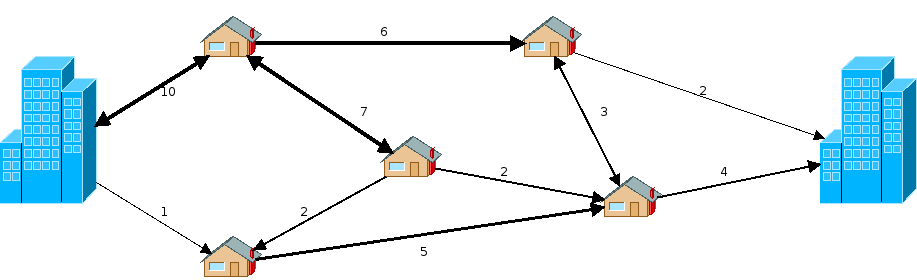
\includegraphics[scale=0.32]{img/exemple.png}
	\end{center}
\end{frame}

\begin{frame}{Sur le graphe de départ}
	$\dots$ et associons lui un graphe.\vfill
	\begin{center}
		\begin{tikzpicture}
			\tikzset{noeud/.style={circle, draw=black, inner sep=0.1cm, minimum width=0.6cm}, fleche/.style={>=latex, ->}};

				\node[noeud] (s) at (0,0) {s};
				\node[noeud] (a) at (2, 2) {a};
				\node[noeud] (b) at (2, -2) {b};
				\node[noeud] (d) at (4.5, -2) {d};
				\node[noeud] (c) at (4.5, 2) {c};
				\node[noeud] (t) at (6.5,0) {t};

				\draw[fleche] (s) to node[above  left] {$5$} (a);
				\draw[fleche] (s) to node[below  left] {$1$} (b);
				\draw[fleche] (a) to node[       left] {$1$} (b);
				\draw[fleche] (a) to node[above      ] {$3$} (c);
				\draw[fleche] (b) to node[below      ] {$1$} (d);
				\draw[fleche] (c) to node[above  left] {$1$} (b);
				\draw[fleche] (c) to node[above right] {$4$} (t);
				\draw[fleche] (d) to node[      right] {$2$} (c);
				\draw[fleche] (d) to node[below right] {$1$} (t);

		\end{tikzpicture}
	\end{center}
\end{frame}

\begin{frame}{Initialisation}
	\begin{minipage}[c]{0.6\linewidth}
		\begin{tikzpicture}[scale=0.55]
			\tikzset{noeud/.style={circle, draw=black, inner sep=0.1cm, minimum width=0.6cm}, fleche/.style={>=latex, ->}};

						\node[noeud] (s1) at (   0,    0) {s};
			\node[noeud] (b1) at (  -2,   -3) {b};
			\node[noeud] (a1) at (   2,   -3) {a};
			\node[noeud] (d1) at (  -2,   -8) {d};
			\node[noeud] (c1) at (   2,   -8) {c};
			\node[noeud] (t1) at (   0,  -11) {t};

			\node[noeud] (s2) at (   8,    0) {s};
			\node[noeud] (b2) at (	 6,   -3) {b};
			\node[noeud] (a2) at (   10,   -3) {a};
			\node[noeud] (d2) at (   6,   -8) {d};
			\node[noeud] (c2) at (   10,   -8) {c};
			\node[noeud] (t2) at (   8,  -11) {t};

			\node at (0,-13) {Graphe de préflot};
			\node at (7,-13) {Réseau résiduel};


			\draw[fleche] (s1) to node[above right] {$0/5$} (a1);
			\draw[fleche] (s1) to node[above  left] {$0/1$} (b1);
			\draw[fleche] (a1) to node[above      ] {$0/1$} (b1);
			\draw[fleche] (a1) to node[      right] {$0/3$} (c1);
			\draw[fleche] (b1) to node[       left] {$0/1$} (d1);
			\draw[fleche] (c1) to node[above right] {$0/1$} (b1);
			\draw[fleche] (c1) to node[below right] {$0/2$} (t1);
			\draw[fleche] (d1) to node[below      ] {$0/2$} (c1);
			\draw[fleche] (d1) to node[below  left] {$0/1$} (t1);

			\draw[fleche] (s2) to node[above right] {$2$} (a2);
			\draw[fleche] (s2) to node[above  left] {$1$} (b2);
			\draw[fleche] (a2) to node[      right] {$3$} (c2);
			\draw[fleche] (b2) to node[       left] {$1$} (d2);
			\draw[fleche] (c2) to node[below right] {$4$} (t2);
			\draw[fleche] (d2) to node[below  left] {$1$} (t2);

		\end{tikzpicture}
	\end{minipage}\hfill
	\begin{minipage}[c]{0.3\linewidth}
		\begin{tabular}{|c|c|c|}
			\hline
			$i$ & $e(i)$ & $d(i)$ \\ \hline
			s & $\infty$ & 6* \\ \hline
			a &  0 & 2 \\ \hline
			b &  0 & 2 \\ \hline
			c &  0 & 1 \\ \hline
			d &  0 & 1 \\ \hline
			t &  0 & 0 \\ \hline
		\end{tabular}
	\end{minipage}
\end{frame}

\begin{frame}{Phase 1}
	\begin{minipage}[c]{0.6\linewidth}
		\begin{tikzpicture}[scale=0.55]
			\tikzset{noeud/.style={circle, draw=black, inner sep=0.1cm, minimum width=0.6cm}, fleche/.style={>=latex, ->}};

						\node[noeud] (s1) at (   0,    0) {s};
			\node[noeud] (b1) at (  -2,   -3) {b};
			\node[noeud] (a1) at (   2,   -3) {a};
			\node[noeud] (d1) at (  -2,   -8) {d};
			\node[noeud] (c1) at (   2,   -8) {c};
			\node[noeud] (t1) at (   0,  -11) {t};

			\node[noeud] (s2) at (   8,    0) {s};
			\node[noeud] (b2) at (	 6,   -3) {b};
			\node[noeud] (a2) at (   10,   -3) {a};
			\node[noeud] (d2) at (   6,   -8) {d};
			\node[noeud] (c2) at (   10,   -8) {c};
			\node[noeud] (t2) at (   8,  -11) {t};

			\node at (0,-13) {Graphe de préflot};
			\node at (7,-13) {Réseau résiduel};


			\draw[fleche, red] (s1) to node[above right, red] {$5/5$} (a1);
			\draw[fleche, red] (s1) to node[above  left, red] {$1/1$} (b1);
			\draw[fleche] (a1) to node[above      ] {$0/1$} (b1);
			\draw[fleche] (a1) to node[      right] {$0/3$} (c1);
			\draw[fleche] (b1) to node[       left] {$0/1$} (d1);
			\draw[fleche] (c1) to node[above right] {$0/1$} (b1);
			\draw[fleche] (c1) to node[below right] {$0/2$} (t1);
			\draw[fleche] (d1) to node[below      ] {$0/2$} (c1);
			\draw[fleche] (d1) to node[below  left] {$0/1$} (t1);

			\draw[fleche] (a2) to node[      right] {$3$} (c2);
			\draw[fleche] (b2) to node[       left] {$1$} (d2);
			\draw[fleche] (c2) to node[below right] {$4$} (t2);
			\draw[fleche] (d2) to node[below  left] {$1$} (t2);

		\end{tikzpicture}
	\end{minipage}\hfill
	\begin{minipage}[c]{0.3\linewidth}
		\begin{tabular}{|c|c|c|}
			\hline
			$i$ & $e(i)$ & $d(i)$ \\ \hline
			s & $\infty$ & 6* \\ \hline
			a &  \textcolor{green}{5} & 2 \\ \hline
			b &  \textcolor{green}{1} & 2 \\ \hline
			c &  0 & 1 \\ \hline
			d &  0 & 1 \\ \hline
			t &  0 & 0 \\ \hline
		\end{tabular}
	\end{minipage}
\end{frame}

\begin{frame}{Phase 1}
	\begin{minipage}[c]{0.6\linewidth}
		\begin{tikzpicture}[scale=0.55]
			\tikzset{noeud/.style={circle, draw=black, inner sep=0.1cm, minimum width=0.6cm}, fleche/.style={>=latex, ->}};

						\node[noeud] (s1) at (   0,    0) {s};
			\node[noeud] (b1) at (  -2,   -3) {b};
			\node[noeud] (a1) at (   2,   -3) {a};
			\node[noeud] (d1) at (  -2,   -8) {d};
			\node[noeud] (c1) at (   2,   -8) {c};
			\node[noeud] (t1) at (   0,  -11) {t};

			\node[noeud] (s2) at (   8,    0) {s};
			\node[noeud] (b2) at (	 6,   -3) {b};
			\node[noeud] (a2) at (   10,   -3) {a};
			\node[noeud] (d2) at (   6,   -8) {d};
			\node[noeud] (c2) at (   10,   -8) {c};
			\node[noeud] (t2) at (   8,  -11) {t};

			\node at (0,-13) {Graphe de préflot};
			\node at (7,-13) {Réseau résiduel};


			\draw[fleche, red] (s1) to node[above right, red] {$5/5$} (a1);
			\draw[fleche, red] (s1) to node[above  left, red] {$1/1$} (b1);
			\draw[fleche] (a1) to node[above      ] {$0/1$} (b1);
			\draw[fleche, red] (a1) to node[      right, red] {$3/3$} (c1);
			\draw[fleche, red] (b1) to node[       left, red] {$1/1$} (d1);
			\draw[fleche] (c1) to node[above right] {$0/1$} (b1);
			\draw[fleche] (c1) to node[below right] {$0/2$} (t1);
			\draw[fleche] (d1) to node[below      ] {$0/2$} (c1);
			\draw[fleche] (d1) to node[below  left] {$0/1$} (t1);

			\draw[fleche] (c2) to node[below right] {$4$} (t2);
			\draw[fleche] (d2) to node[below  left] {$1$} (t2);

		\end{tikzpicture}
	\end{minipage}\hfill
	\begin{minipage}[c]{0.3\linewidth}
		\begin{tabular}{|c|c|c|}
			\hline
			$i$ & $e(i)$ & $d(i)$ \\ \hline
			s & $\infty$ & 6* \\ \hline
			a &  \textcolor{orange}{2} & 2 \\ \hline
			b &  \textcolor{orange}{0} & 2 \\ \hline
			c &  \textcolor{green}{3} & 1 \\ \hline
			d &  \textcolor{green}{1} & 1 \\ \hline
			t &  0 & 0 \\ \hline
		\end{tabular}
	\end{minipage}
\end{frame}


\subsection{Les algorithmes dérivés}

\begin{frame}{Une question de choix}
	Les algorithmes dérivés sont basés sur un choix plus judicieux des sommets actfis à traiter.
	\vfill
\end{frame}

\begin{frame}{Une question de choix}
	Les algorithmes dérivés sont basés sur un choix plus judicieux des sommets actfis à traiter.
	\vfill
	\textbf{L'algorithme FIFO :} dès qu'un noeud devient actif, on le place dans une file. On traite
	alors les sommets de la file dans l'ordre \emph{First In First Out}\vfill
\end{frame}

\begin{frame}{Une question de choix}
	Les algorithmes dérivés sont basés sur un choix plus judicieux des sommets actfis à traiter.
	\vfill
	\textbf{L'algorithme FIFO :} dès qu'un noeud devient actif, on le place dans une file. On traite
	alors les sommets de la file dans l'ordre \emph{First In First Out}\vfill
	\textbf{L'algorithme High Label :} on choisit de préférence, le noeud actif ayant la plus grande
	distance au puits \vfill
\end{frame}

\begin{frame}{Complexités}
	\renewcommand{\arraystretch}{2.5}
	\begin{tabular}{c|p {0.12\linewidth}|p {0.35\linewidth}|p {0.35\linewidth}|} \cline{3-4}
		\multicolumn{2}{c|}{}& Algorithme & Complexité \\ \cline{2-4}
		&\multirow{2}{*}{$\quad$\rotatebox{90}{\parbox[b]{5.1em}{\centering Chaînes\\ améliorantes~}}} & Edmonds-Karp & $O(SA^2)$ \\
		\cline{3-4}
	\renewcommand{\arraystretch}{2}
		& & Dinic & $O(S^2A)$ \\\cline{2-4}
		&\multirow{3}{*}{$\quad$\rotatebox{90}{\parbox[t]{5.5em}{\centering Poussage\\ Réétiquetage}}} &
		Générique & $O(S^2A)$ \\ \cline{3-4}
		& & FIFO & $O(S^3)$ \\ \cline{3-4}
		& & High Label & $O(S^2\sqrt{A})$ \\ \cline{2-4}
	\end{tabular}
\end{frame}




\section{Les tests}

\subsection{Modus Operandi}

\begin{frame}{Les tests}
	\begin{itemize}
		\item Définit la densité : $r = \frac{m}{n}$
	\end{itemize}
\end{frame}

\begin{frame}{Les tests}
	\begin{itemize}
		\item Définit la densité : $r = \frac{m}{n}$
		\item Fait varier le nombre de noeuds
	\end{itemize}
\end{frame}
\begin{frame}{Les tests}
	\begin{itemize}
		\item Définit la densité : $r = \frac{m}{n}$
		\item Fait varier le nombre de noeuds
		\item Réalise les trois algorithmes sur 100 graphes aléatoires différents
	\end{itemize}
\end{frame}
\begin{frame}{Les tests}
	\begin{itemize}
		\item Définit la densité : $r = \frac{m}{n}$
		\item Fait varier le nombre de noeuds
		\item Réalise les trois algorithmes sur 100 graphes aléatoires différents
		\item Trace les courbes
	\end{itemize}
\end{frame}

\subsection{Retour d'expériences}

\begin{frame}{Les résultats attendus}
	Pour une densité $r = O(n^2)$ : 
\end{frame}

\begin{frame}{Les résultats attendus}
	Pour une densité $r = O(n^2)$ : \begin{itemize}
		\item Une complexité en $O(n^4)$ pour Dinic
	\end{itemize}
\end{frame}

\begin{frame}{Les résultats attendus}
	Pour une densité $r = O(n^2)$ : \begin{itemize}
		\item Une complexité en $O(n^4)$ pour Dinic
		\item Une complexité en $O(n^3)$ pour les algorithmes FIFO et High Label
	\end{itemize}
\end{frame}

\begin{frame}{Les résultats attendus}
	Pour une densité $r = O(n^2)$ : \begin{itemize}
		\item Une complexité en $O(n^4)$ pour Dinic
		\item Une complexité en $O(n^3)$ pour les algorithmes FIFO et High Label
		\item Une exécution plus rapide pour FIFO et High Label
	\end{itemize}
\end{frame}

\begin{frame}{Les résultats obtenus}
	\begin{center}
	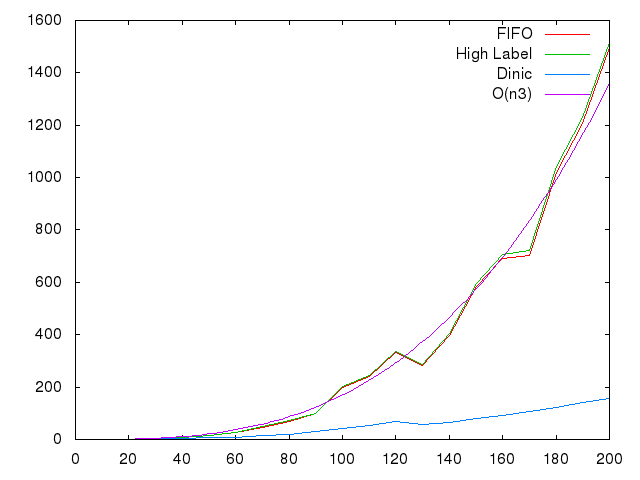
\includegraphics{img/resultat.png}
	\end{center}
\end{frame}


\begin{frame}{Les résultats obtenus}
	\begin{minipage}[c]{0.50\linewidth}
		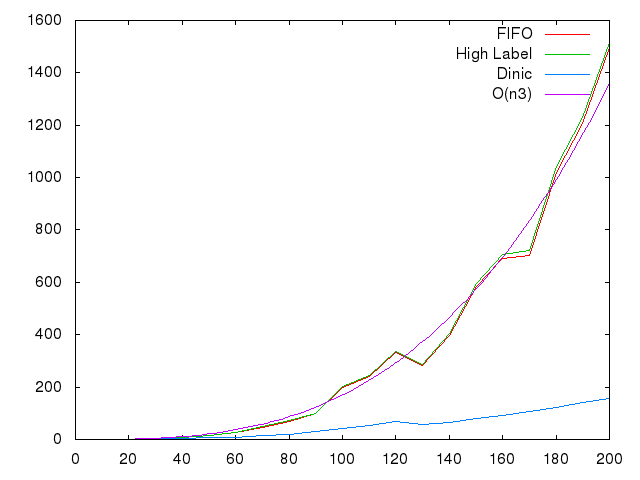
\includegraphics[scale=0.6]{img/resultat.png}
	\end{minipage}\hfill
	\begin{minipage}[c]{0.40\linewidth}
	\end{minipage}
\end{frame}

\begin{frame}{Les résultats obtenus}
	\begin{minipage}[c]{0.50\linewidth}
		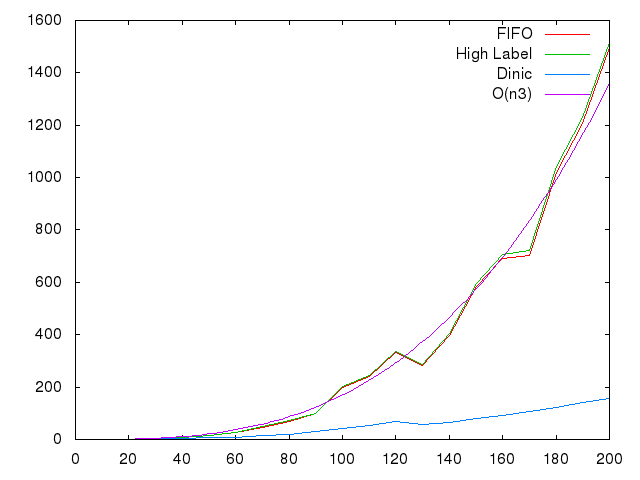
\includegraphics[scale=0.6]{img/resultat.png}
	\end{minipage}\hfill
	\begin{minipage}[c]{0.40\linewidth}
		\begin{itemize}
			\item $O(n^4)$ pour Dinic
			\end{itemize}
	\end{minipage}
\end{frame}

\begin{frame}{Les résultats obtenus}
	\begin{minipage}[c]{0.50\linewidth}
		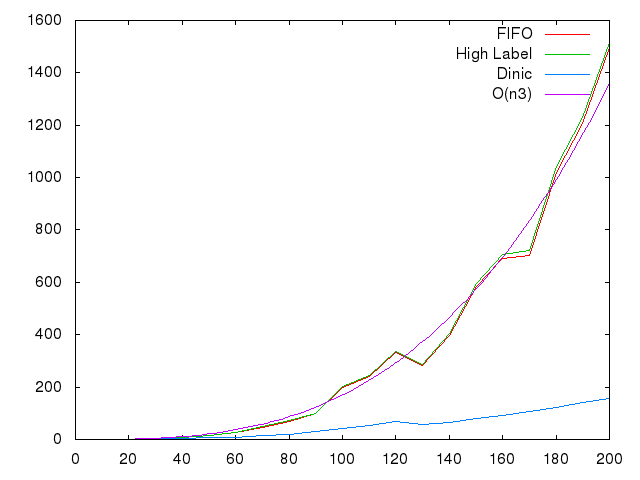
\includegraphics[scale=0.6]{img/resultat.png}
	\end{minipage}\hfill
	\begin{minipage}[c]{0.40\linewidth}
		\begin{itemize}
			\item $O(n^4)$ pour Dinic
			\item $O(n^3)$ pour les algorithmes de préflots
		\end{itemize}
	\end{minipage}
\end{frame}

\begin{frame}{Les résultats obtenus}
	\begin{minipage}[c]{0.50\linewidth}
		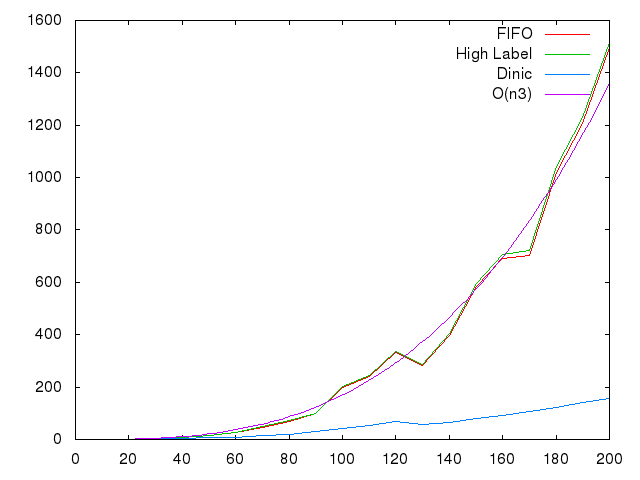
\includegraphics[scale=0.6]{img/resultat.png}
	\end{minipage}\hfill
	\begin{minipage}[c]{0.40\linewidth}
		\begin{itemize}
			\item $O(n^4)$ pour Dinic
			\item $O(n^3)$ pour les algorithmes de préflots
			\item Un temps égal pour les algorithmes de préflots
		\end{itemize}
	\end{minipage}
\end{frame}



\section{Conclusion}

\begin{frame}{Conclusion}
	\begin{itemize}
		\item Algorithmes intéressants (complexités, principes, fonctions de préflots, ...)
	\end{itemize}
\end{frame}

\begin{frame}{Conclusion}
	\begin{itemize}
		\item Algorithmes intéressants (complexités, principes, fonctions de préflots, ...)
		\item Parmis les plus rapides en pratique et en théorie
	\end{itemize}
\end{frame}

\end{document}
